\chapter{Model Design and Implementation}
\label{chap:model-design-and-implementation}

The processed WeChat behavioural records, article files, and agent profile data provide the analysis-ready variables used in the empirical models. The variable role map specifies how each variable may enter the analysis, and the model design builds on that map to answer the three research questions.

Figure 5.1 summarises the three-level modelling framework used in this chapter. The Level 1 article–agent cases form the base unit, while the Level 2 and Level 3 datasets are constructed by aggregating those cases over agents and over agent–topic combinations. This structure keeps the research questions aligned with the level at which their predictors and outcomes are observed.

\begin{figure}[H]
\centering
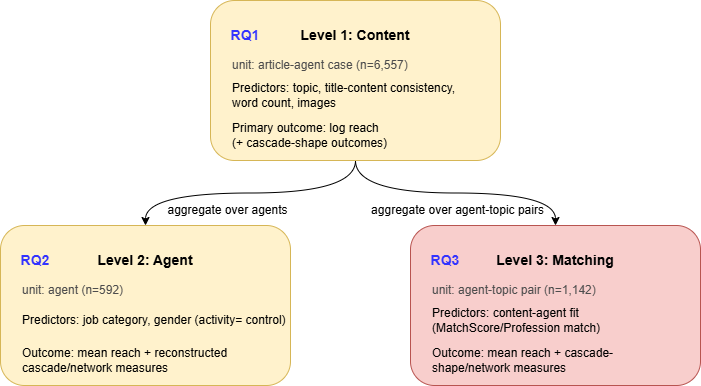
\includegraphics[width=0.86\textwidth]{figures/figure_5_1_three_level_framework.png}
\caption{Three-level empirical modelling framework.}
\label{fig:5-1}
\end{figure}

\section{Level 1 Content Model}
\label{sec:5-1-level-1-content-model}

The Level 1 model addresses the first research question: whether observable article content characteristics are associated with diffusion effectiveness. Its purpose is to establish a content-only baseline that describes how articles with different content properties diffuse, before any agent-characteristic or content–agent matching variables are introduced. The unit of analysis is the article–agent diffusion case, so that one observation corresponds to a single article shared by a single agent together with the cascade that this share generated.

The primary outcome is \varname{log\_reach}, the log-transformed reach of the article–agent cascade. The main specification regresses this outcome on the article's content topic and its content-format and semantic-consistency features:
\begin{equation}
\begin{aligned}
\varname{log\_reach}_{ij}
={}& \beta_{0}
+ \gamma' \varname{TopContentCluster}_{i}
+ \beta_{1}\varname{z\_CosineSim}_{i} \\
&+ \beta_{2}\varname{z\_WordCount}_{i}
+ \beta_{3}\varname{HasImage}_{i}
+ \beta_{4}\varname{z\_NumImages}_{i}
+ \varepsilon_{ij}.
\end{aligned}
\end{equation}

where i indexes the article and j the agent-sharing case. These predictors represent four dimensions of article content: substantive topic (\varname{TopContentCluster}), title–content semantic consistency (\varname{CosineSim}), textual length (\varname{WordCount}), and visual presentation (\varname{HasImage} and \varname{NumImages}). \varname{TopContentCluster} enters as a categorical predictor whose six canonical topic categories are estimated through indicator contrasts relative to a single reference category, so that γ captures each topic's difference from the baseline. \varname{CosineSim}, the title–content semantic consistency measure, is the central content predictor of interest. The continuous predictors are standardised before estimation, denoted by the z\_ prefix, so that their coefficients are directly comparable as standardised effects measured on a common scale. \varname{HasImage}, being binary, enters untransformed. The six topic-probability scores are not entered alongside the topic dummies in the main model, because the dominant-topic category and the underlying scores represent the same information at different resolutions. The scores are reserved for the robustness specifications described below.

The model is estimated by ordinary least squares with heteroskedasticity-robust (HC3) standard errors. The main complete-case sample contains 6,556 article–agent cases, one fewer than the 6,557-row master dataset, because a single very short article lacks a defined \varname{CosineSim} value and is dropped from the specifications that include it.

\section{Level 2 Agent-Characteristic Model}
\label{sec:5-2-level-2-agent-characteristic-model}

The Level 2 model addresses the second research question: whether observable agent characteristics are associated with agent-level diffusion patterns. Its purpose is to examine whether agents differ systematically in their average diffusion performance, and whether such differences are associated with observable attributes of the agent instead of the content of any particular article. The unit of analysis is the agent, so one observation aggregates all of an agent's article–agent cases into a summary of that agent's typical diffusion behaviour.

Aggregation to the agent is what gives the reconstructed cascade and network measures a coherent meaning at this level. A quantity such as an agent's average cascade size or average centrality describes an average pattern across that agent's observed sharing activity; the same quantity computed for a single share would not carry the same interpretation. Since each agent is both an embedded member of a social network and the origin point from which diffusion begins, the agent's observable attributes are interpreted as proxies for the local audience and sharing context that the agent represents.

The primary outcome is \varname{log\_agent\_cascade\_size\_mean}, the log-transformed mean cascade size across the article–agent cases belonging to an agent. The main specification regresses this outcome on the agent's observable role and demographic attributes, together with a control for the agent's activity level:
{\setlength{\abovedisplayskip}{0pt}
\setlength{\belowdisplayskip}{0.35\baselineskip}
\setlength{\abovedisplayshortskip}{0pt}
\setlength{\belowdisplayshortskip}{0.35\baselineskip}
\begin{equation}
\begin{aligned}
&\varname{log\_agent\_cascade\_size\_mean}_{a} \\
&\quad= \beta_{0}
+ \gamma' \varname{JobCategory}_{a}
+ \delta' \varname{agent\_gender}_{a} \\
&\qquad
+ \beta_{1}\varname{z\_log\_article\_count\_per\_agent}_{a}
+ \varepsilon_{a}.
\end{aligned}
\end{equation}
}
where a indexes the agent. \varname{JobCategory} enters as a categorical predictor. Of the five role categories, the Unknown category contains a single agent and is excluded from the fitted role model, because contrasts involving a single-agent category would be too imprecise to interpret. The four remaining roles, Marketing/Operations, Design, Field Sales, and Online Sales/Customer Service, are estimated through indicator contrasts relative to Field Sales, the largest category. The coefficient vector γ captures each role's difference from the field-sales baseline. The \varname{agent\_gender} variable enters as a categorical attribute. The agent's activity level, \varname{log\_article\_count\_per\_agent}, is included as an exposure and stability control: agents who share more articles both have more opportunities to generate reach and have more stable average outcomes. Controlling for activity helps distinguish role or gender associations from differences in observed sharing volume. The control is log-transformed because the number of shares per agent is highly skewed, and it is standardised before estimation, denoted by the z\_ prefix, so that its coefficient is comparable as a standardised effect.

The model is estimated by ordinary least squares with heteroskedasticity-robust (HC3) standard errors. The fitted core-model sample contains 591 agents, one fewer than the 592-agent master dataset, since the single Unknown-category agent is excluded from the fitted role model. Unlike the content model, the Level 2 framework retains the reconstructed cascade and network-position measures as agent-level supplementary outcomes.

\section{Level 3 Content–Agent Matching Model}
\label{sec:5-3-level-3-content-agent-matching-model}

The Level 3 model addresses the third research question, which is the central concern of the dissertation: whether content–agent fit is associated with diffusion performance. It tests whether stronger alignment between an article's topics and the sharing agent's professional context is associated with stronger diffusion. This provides the most direct empirical test of the proposition that, in agent-based social marketing, one size does not fit all.

The unit of analysis is the agent–topic pair, so one observation aggregates the article–agent cases falling within a particular combination of an agent and a content topic. This unit isolates how a given topic performed when shared by a given agent context. It also keeps the topic-specific matching relationship separate from the article-level content model and the whole-agent model.

The primary outcome is \varname{log\_agent\_topic\_cascade\_size\_mean}, the log-transformed mean cascade size within an agent–topic pair. Content–agent fit is operationalised through two matching measures constructed during dataset assembly: \varname{MatchScore\_mean}, the average continuous fit score between an agent and a content topic across the cases in the pair, and \varname{ProfessionContentMatch\_mean}, the proportion of cases in the pair classified as professionally matched. These two measures capture the same underlying construct at different resolutions. They are estimated in two separate core specifications and are not entered together. The two specifications are defined as follows.
{\setlength{\abovedisplayskip}{0pt}
\setlength{\belowdisplayskip}{0.35\baselineskip}
\setlength{\abovedisplayshortskip}{0pt}
\setlength{\belowdisplayshortskip}{0.35\baselineskip}
\begin{align}
\begin{split}
\text{Model A:}\quad
&\varname{log\_agent\_topic\_cascade\_size\_mean}_{at} \\
={}& \beta_{0}
+ \beta_{1}\varname{z\_MatchScore\_mean}_{at}
+ \theta' \varname{Controls}_{at}
+ \varepsilon_{at},
\end{split} \\
\begin{split}
\text{Model B:}\quad
&\varname{log\_agent\_topic\_cascade\_size\_mean}_{at} \\
={}& \beta_{0}
+ \beta_{1}\varname{z\_ProfessionContentMatch\_mean}_{at}
+ \theta' \varname{Controls}_{at}
+ \varepsilon_{at}.
\end{split}
\end{align}
}
Here, a indexes the agent and t the content topic, and the control vector \varname{Controls} is identical across the two models. In each specification the matching measure is the predictor of interest and is standardised before estimation, denoted by the z\_ prefix, so that its coefficient is comparable as a standardised effect. \varname{MatchScore\_mean} preserves variation in the intensity of alignment. It captures how strongly the topic profile of the shared articles aligns with the professional relevance profile of the agent's job category. \varname{ProfessionContentMatch\_mean} is derived from the binary article–agent matching indicator and then averaged within the pair. At Level 3 it is a proportion, not a binary variable: a value close to one indicates that most cases in the cell are professionally matched, while a value close to zero indicates that few are.

The control vector comprises \varname{TopContentCluster} and \varname{JobCategory} as categorical controls, \varname{agent\_gender} as a categorical attribute, the log-transformed and standardised exposure control \varname{z\_log\_agent\_topic\_article\_n} for the number of cases in the pair, and the aggregated content controls \varname{z\_WordCount\_mean}, \varname{z\_HasImage\_share}, \varname{z\_NumImages\_mean}, and \varname{z\_CosineSim\_mean}. The topic-category contrasts use Home Design \& Decoration as the reference category, matching the Level 1 content models. Including the aggregated content controls helps interpret the matching coefficient net of the article-format and semantic-consistency characteristics of the content shared within the pair. In particular, \varname{z\_CosineSim\_mean} adjusts for average title–content consistency within the agent–topic cell, so that the matching measure is not capturing content coherence already examined at Level 1.

The models are estimated by ordinary least squares with heteroskedasticity-robust (HC3) standard errors. The main complete-case sample contains 1,142 agent–topic pairs. As at the other levels, the same two matching specifications are also estimated against supplementary agent–topic outcomes that capture cascade shape and reconstructed network position beyond reach.

\section{Supplementary Outcome Models and Robustness Design}
\label{sec:5-4-supplementary-outcome-models-and-robustness-design}

Because diffusion effectiveness is multi-dimensional, each level's core specification is re-estimated against supplementary outcomes that describe the shape and engagement pattern of diffusion beyond reach. These models retain the same predictors as the corresponding core model but use different dependent variables, so each coefficient shows which diffusion dimension a predictor is associated with. The robustness specifications test whether each level's core findings depend on particular modelling choices. All estimated coefficients, family-specific fit statistics, robustness comparisons, and diagnostics are reported in Chapter~\ref{chap:empirical-results}, with the complete coefficient tables for the supplementary outcomes provided in Appendix~\ref{app:supplementary-regression-results}.

At Level 1, the supplementary outcomes are the article–agent cascade-shape dimensions: cascade depth, the reshare proportion, reading duration, structural virality, and the Wiener index, together with second-layer width as a count outcome. The structural-virality and Wiener-index measures are heavy-tailed across cascades, so each is winsorised at its 99th percentile before estimation to limit the influence of a small number of extreme cascades. These continuous outcomes are estimated by ordinary least squares. Whether any resharing occurred within a cascade is a binary outcome and is modelled by logistic regression. The count outcomes, cascade size and second-layer width, are modelled by negative binomial regression, which accommodates over-dispersion.

The robustness design at this level targets the two content choices most likely to influence the content findings: how topic is represented and how semantic consistency is measured. First, the dominant-topic dummies are replaced by the standardised six-cluster content topic-probability scores, with the reference topic's score held out, so that topic enters as a continuous distribution instead of a single assigned category. Second, the topic-probability scores are reduced to a small number of principal components, up to three, which are entered in place of the dummies. This guards against any artefact arising from how the dominant category was coded. Third, the semantic-consistency measure \varname{CosineSim} is replaced in turn by the two alternative title–content distance measures, \varname{EuclideanDist} and \varname{ManhattanDist}. Because these measures increase as the title and content diverge, a consistency finding should appear with the opposite sign under the distance measures, confirming that it is not specific to the cosine definition. These three robustness specifications are applied across the full set of Level 1 outcomes, not only reach. Fourth, the main specification is re-estimated with standard errors clustered on the agent and, separately, on the article. The same agent shares many articles and the same article is shared by many agents, so residuals are likely to be correlated within these groupings. A condition-number diagnostic on the continuous content predictors is also reported to confirm that they are not collinear.

At Level 2, the supplementary outcomes are agent-level averages of the reconstructed cascade and network measures. They include mean cascade depth, the mean reshare proportion, mean second-layer width, mean structural virality, the mean Wiener index, the centrality-class measures, the first- and second-layer repeat-exposure proportions, gender assortativity, and mean reading duration. Each outcome is estimated by ordinary least squares using the same agent-attribute predictors as the core reach model. This allows the agent characteristics to be examined across a full range of agent-level diffusion dimensions. The robustness design re-estimates the core model and each supplementary model without the activity control, \varname{log\_article\_count\_per\_agent}, to confirm that the role and gender associations are not contingent on how much an agent shares. A collinearity diagnostic over the Level 2 agent-level continuous measures is also reported.

At Level 3, the supplementary outcomes are agent–topic averages of cascade depth, the reshare proportion, second-layer width, structural virality, the Wiener index, the centrality-class measures, and reading duration. Each is estimated by ordinary least squares. Both matching specifications are estimated against every supplementary outcome, so content–agent fit is examined across the same range of agent–topic diffusion dimensions as reach.

Two robustness considerations are specific to this level and follow from the way agent–topic pairs are populated. First, because pairs differ in the number of underlying article–agent cases, each specification is also estimated as a weighted regression using the number of underlying cases per pair as exposure weights. Pairs supported by more observed evidence then contribute more to the estimates than thinly populated pairs. Second, the specifications are re-estimated on a less sparse subset, restricting the sample to pairs with at least ten underlying cases, to test whether the findings depend on the many pairs supported by only a few cases. A stricter threshold of thirty cases was also considered. Although forty-six pairs meet it, this subset is too small and too concentrated, with almost all qualifying pairs falling within a single content topic and across only two job categories. It cannot support the full control specification under the pipeline's minimum-sample rule, so no thirty-case model is reported. A diagnostic on the relationship between the two matching measures is also reported, which informs the decision to estimate them separately.

\section{Leakage Control and Estimation Principles}
\label{sec:5-5-leakage-control-and-estimation-principles}

The three-level design is governed by a single principle that determines how every variable may be used: a variable's permitted role depends on whether it exists prior to diffusion or is a product of the diffusion being studied. Content characteristics, agent attributes, and the content–agent matching measures are all defined from article content, agent attributes, or their pre-diffusion alignment, not from realised diffusion outcomes. The article's topic, length, image use, and title–content consistency are properties of the article itself. An agent's job category and gender are properties of the agent. The matching measures are constructed from the agent's professional role and the article's content topic. These variables can serve as predictors.

The reconstructed diffusion and network-position measures are different in kind because they are computed from the same realised cascades that define the diffusion outcomes. Using such a measure to predict reach would explain diffusion through a quantity that is itself a product of that diffusion, producing a coefficient that cannot be interpreted as an ex-ante relationship. These measures are confined to the outcome side of the analysis throughout, appearing only as primary or supplementary outcomes and not as predictors of the diffusion outcomes to which they are mechanically related.

The same principle accounts for the removal of an earlier moderation framing. An initial design had considered using reconstructed network-position measures such as centrality to moderate the association between content characteristics and diffusion, for example by asking whether content effects differed for agents in more central network positions. Under leakage control this is not admissible. A moderator built from the realised cascade would condition the content association on a quantity that is itself an outcome of diffusion, reintroducing on the right-hand side exactly the leakage the design is intended to prevent. The moderation specifications were removed, and the measures involved are retained only as outcomes.

Several estimation conventions are applied uniformly across the three levels. Continuous predictors are standardised before estimation, denoted by the z\_ prefix, so that their coefficients are comparable as standardised effects on a common scale. Binary indicators such as \varname{HasImage} and categorical predictors such as \varname{TopContentCluster}, \varname{JobCategory}, and \varname{agent\_gender} enter without standardisation. Continuous outcomes are estimated by ordinary least squares with heteroskedasticity-robust (HC3) standard errors, with standard errors clustered or estimates weighted where the design requires it. Outcomes whose distributional form departs from continuity are estimated with the appropriate model family described above. Each specification is estimated on the complete cases for its own variable set, so that a model's reported sample size is the number of observations with non-missing values on every term it contains.

A final principle concerns the two matching measures at Level 3. The binary indicator \varname{ProfessionContentMatch} is a deterministic encoding of \varname{MatchScore}: it classifies a case as matched when its continuous fit score clears a fixed threshold. At the agent–topic level, \varname{ProfessionContentMatch\_mean} and \varname{MatchScore\_mean} are two representations of the same underlying construct at different resolutions. Entering both in one regression would place a variable and a deterministic function of that variable on the same right-hand side, producing severe collinearity and coefficients that could not be separately interpreted. The two measures are accordingly estimated in separate specifications, with the continuous measure treated as the primary operationalisation of content–agent fit and the threshold-based proportion treated as an alternative encoding that tests whether a simpler matched-versus-unmatched classification reproduces the same pattern.

\section{Implementation Pipeline and Reproducibility}
\label{sec:5-6-implementation-pipeline-and-reproducibility}

The empirical analysis is implemented as a single, end-to-end pipeline, so that the complete set of results can be regenerated from the source data in one run. The pipeline begins by flagging missing or invalid required inputs before modelling proceeds, so that no analysis is carried out on incomplete data. It then assembles the three level-specific master datasets, standardises the content topic labels into the six canonical categories used throughout the study, and writes out the variable role map that fixes each major variable's permitted modelling role at each empirical level before any model is estimated. With these inputs prepared, the pipeline runs the Level 1, Level 2, and Level 3 analyses in turn, including their supplementary outcome and robustness specifications, and exports the resulting coefficient tables, fit statistics, diagnostics, and figures.

Reproducibility is supported by automatic checks built into the pipeline. The three master datasets are validated against their expected sizes of 6,557 article–agent cases, 592 agents, and 1,142 agent–topic pairs. The run records a validation report, so that any departure from these counts is visible immediately. Fixing the variable roles in advance, validating the dataset sizes, and gating the run on source-file readiness together mean that each regeneration of the results operates on the same data with the same variable definitions.

The full implementation, including the pipeline source code, the test suite, and the generated tables and figures, is retained as reproducibility material. The fuller account of the pipeline's organisation and validation outputs is provided in Appendix~\ref{app:implementation-reproducibility}.
